The Presentation Node serves the static files and scripts to run a single page application (SPA) on the client's browser.
The SPA web interface allows a wide number of interaction without the need of refreshing the page, providing a smoother user experience. The platform root page is the Home Page from which every non-registered user can find information about S\&C such as the latest news. The Home page is linked to other pages, such as the Dashboard, Contacts, and About page, using an app bar. 
In the Contacts page, the user can find useful links to get in touch with S\&C.\\
\begin{figure}[H]
    \centering
    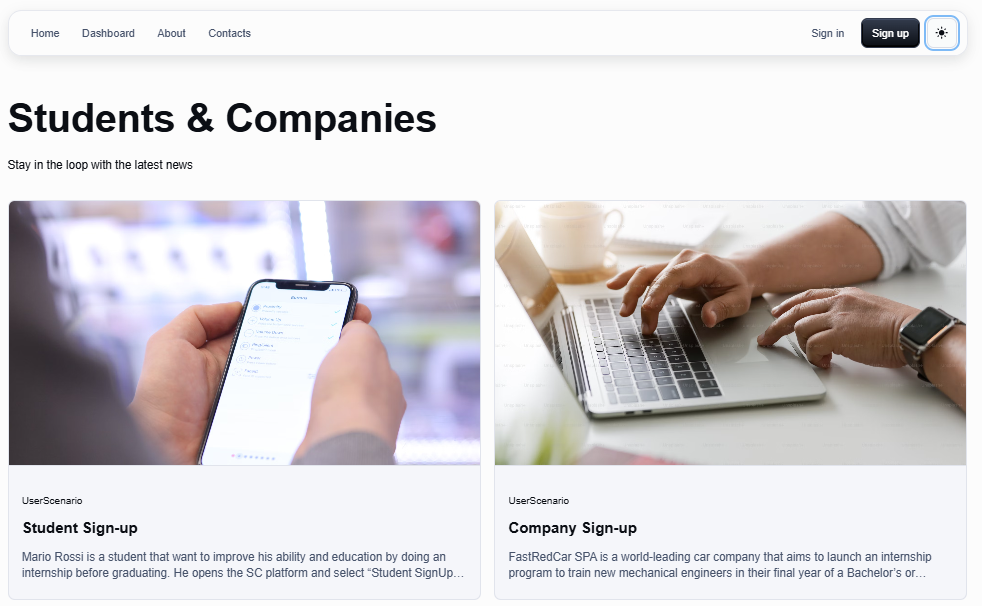
\includegraphics[width=\textwidth]{Latex/Images/HomePage.png}
    \caption{UI Home Page: as an example, UI cards containing some user scenarios described in the \ref{subsec: user scenarios}  are shown}
    \label{fig:homepage}
\end{figure}
\begin{figure}[H]
    \centering
    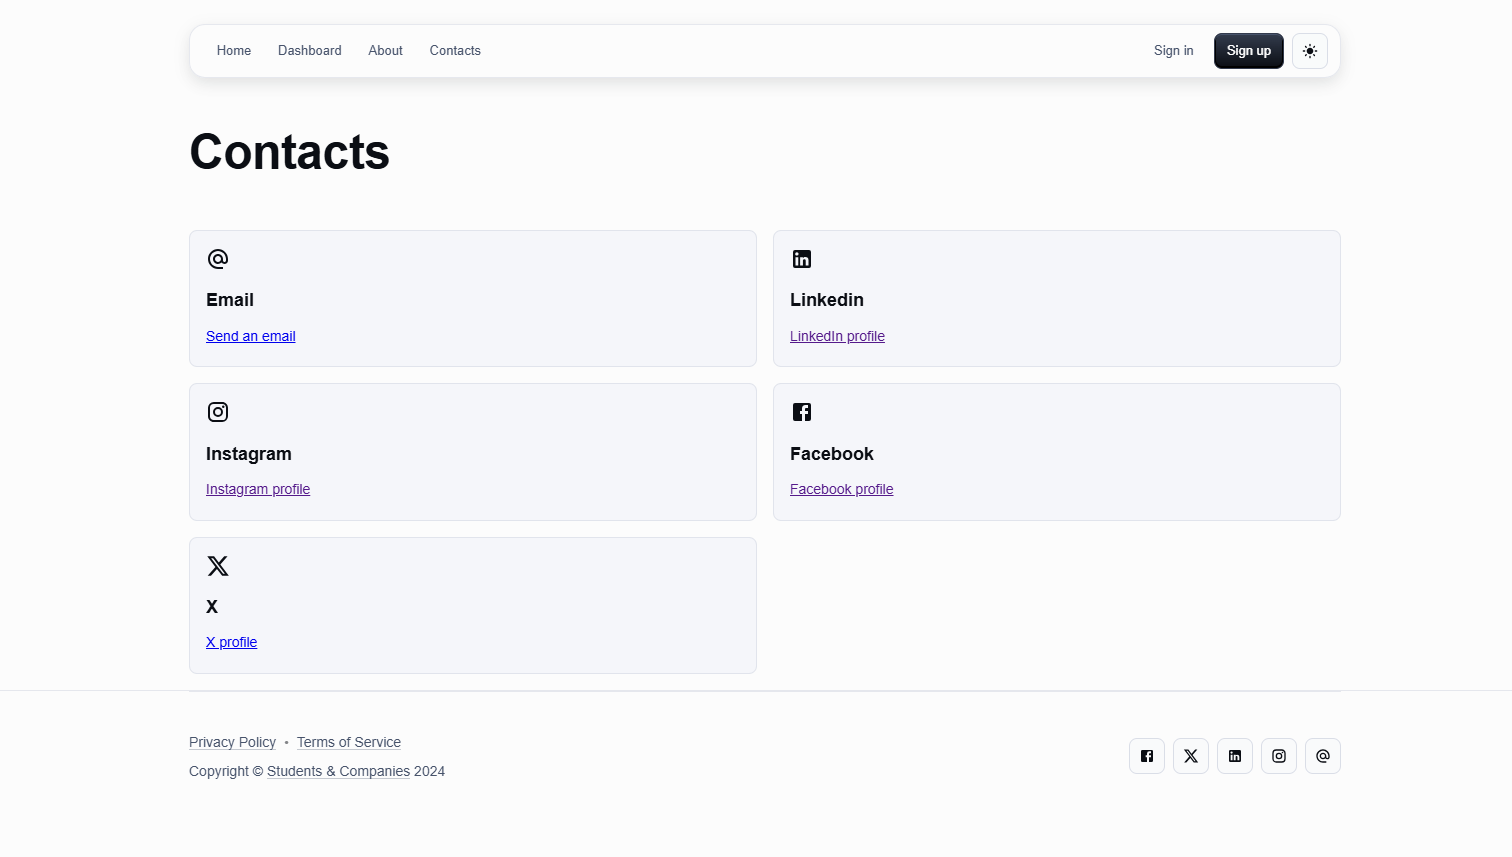
\includegraphics[width=\textwidth]{Latex/Images/New Ui/Contacts.png}
    \caption{UI Contacts Page}
    \label{fig:contactpage}
\end{figure}
\noindent Thanks to the app bar link buttons, users can also reach the Sign-Up and Sign-in pages. The Sign-Up page allows for different types of sign-up according to the new user type. This allows the user to provide the platform with the correct information.
\begin{figure}[H]
    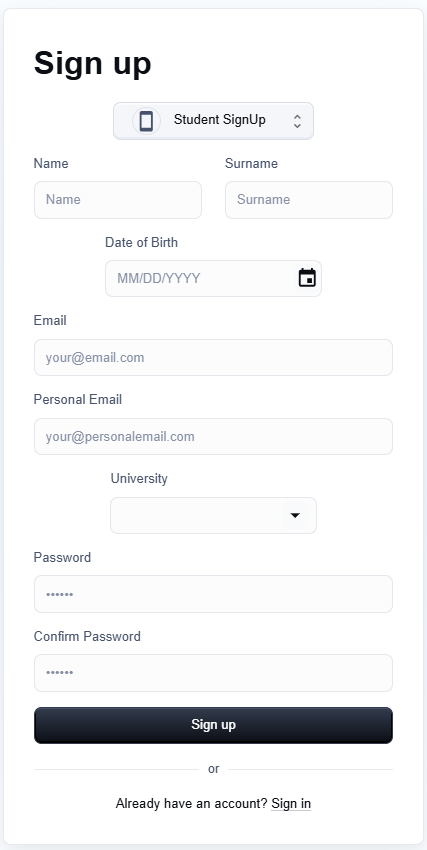
\includegraphics[width=0.33\textwidth]{Latex/Images/New Ui/SignUp Student.png}
    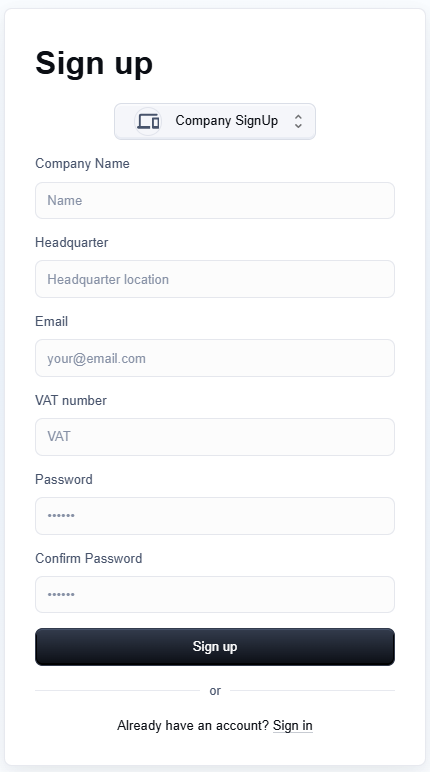
\includegraphics[width=0.33\textwidth]{Latex/Images/New Ui/SignUp Company.png}
    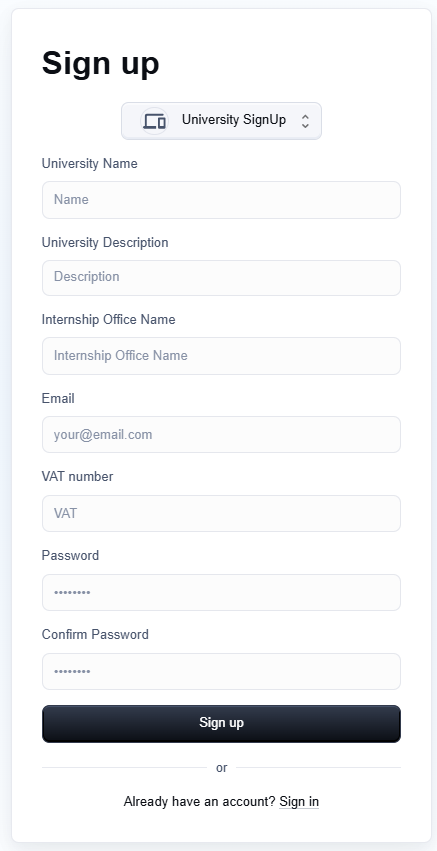
\includegraphics[width=0.33\textwidth]{Latex/Images/New Ui/SignUp University.png}
    \caption{UI Sign-Up Page}
    \label{fig:signuppage}
\end{figure}
To be able to log into the platform, the user shall provide his email and password. 
\begin{figure}[H]
    \centering
    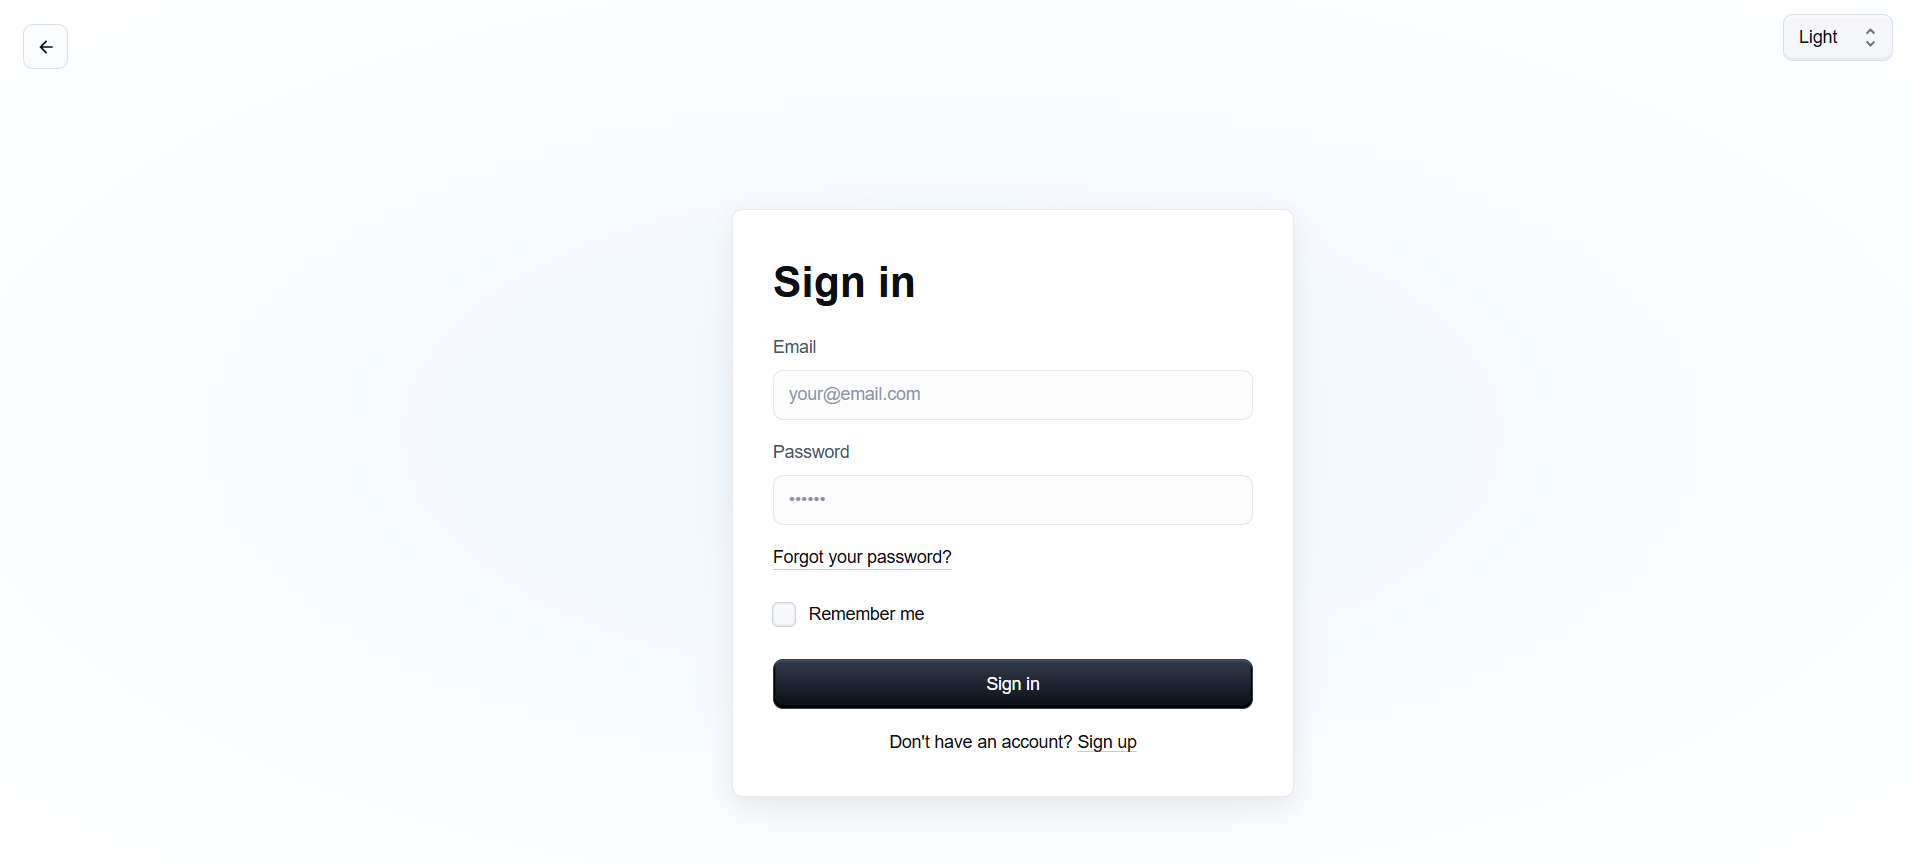
\includegraphics[width=\textwidth]{Latex/Images/New Ui/SignInPage.png}
    \caption{UI Sign-In Page}
    \label{fig:signinpage}
\end{figure}
\noindent The Dashboard page will be the central hub for logged-in users. From the left-hand panel of the dashboard, all the pages associated with the core functionalities of the platform are reachable. Therefore, this page is provided after a successful log-in. The side panel contains different elements according to the user needs.
\begin{figure}[H]
    \centering
    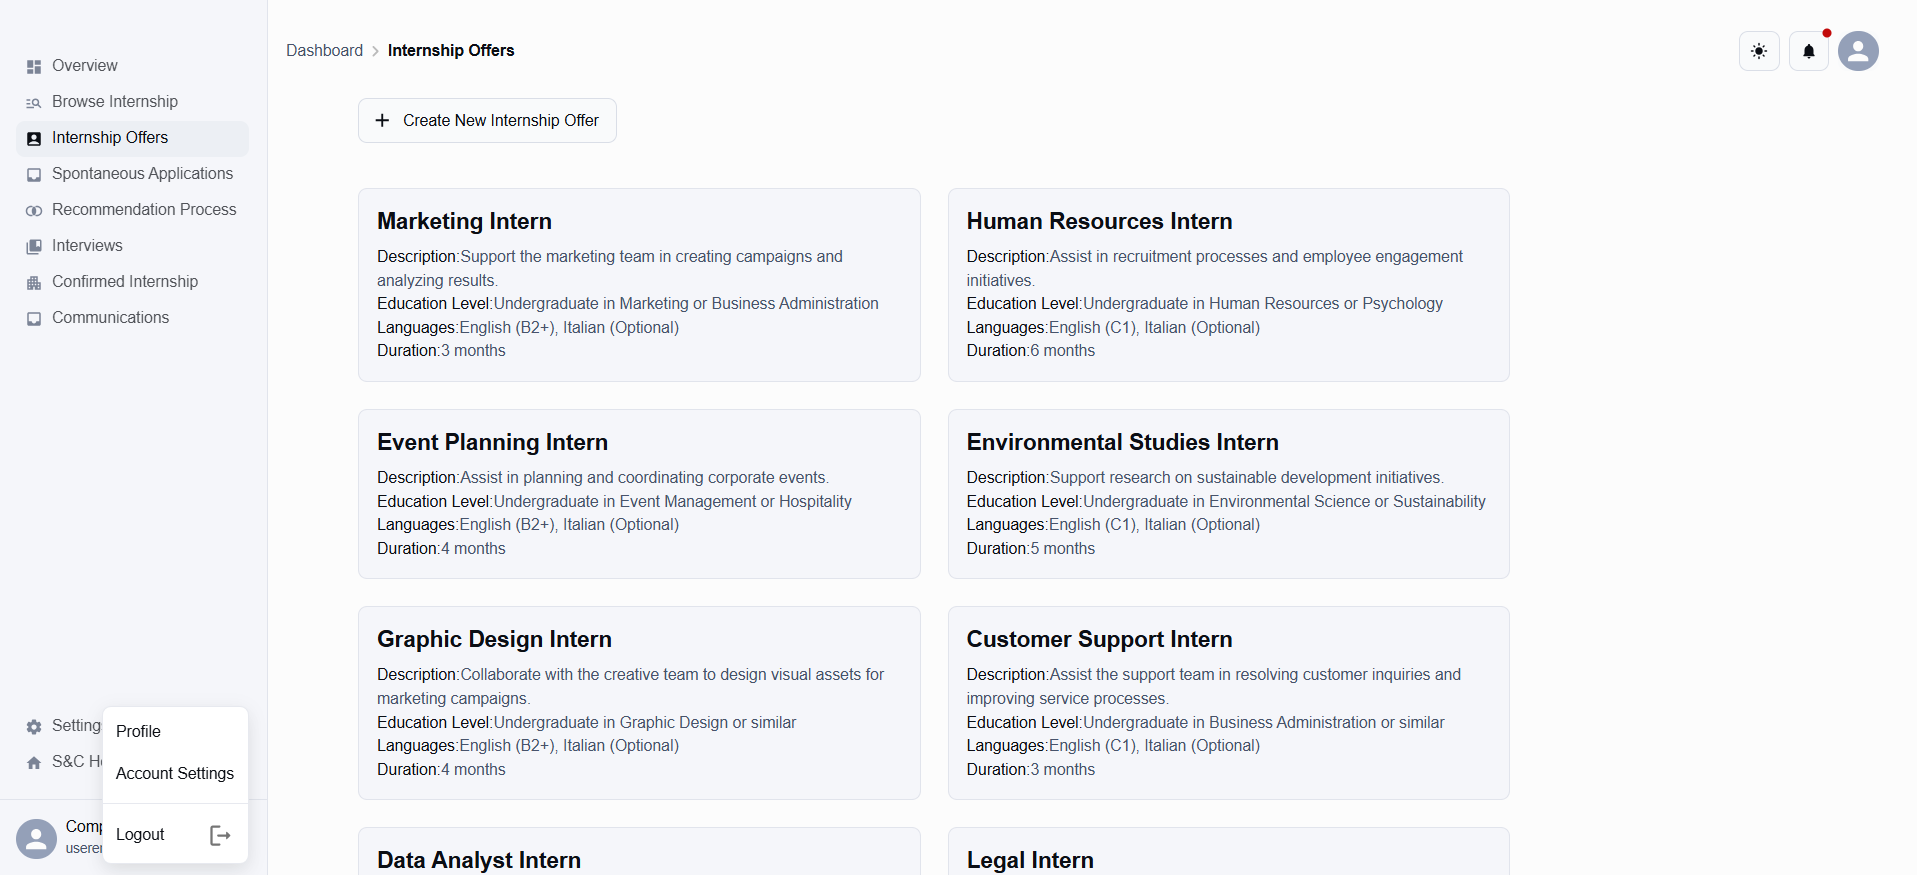
\includegraphics[width=\textwidth]{Latex/Images/New Ui/Company-Dashboard.png}
    \caption{UI Company Dashboard Page}
    \label{fig:companyDashboard}
\end{figure}
\begin{figure}[H]
    \centering
    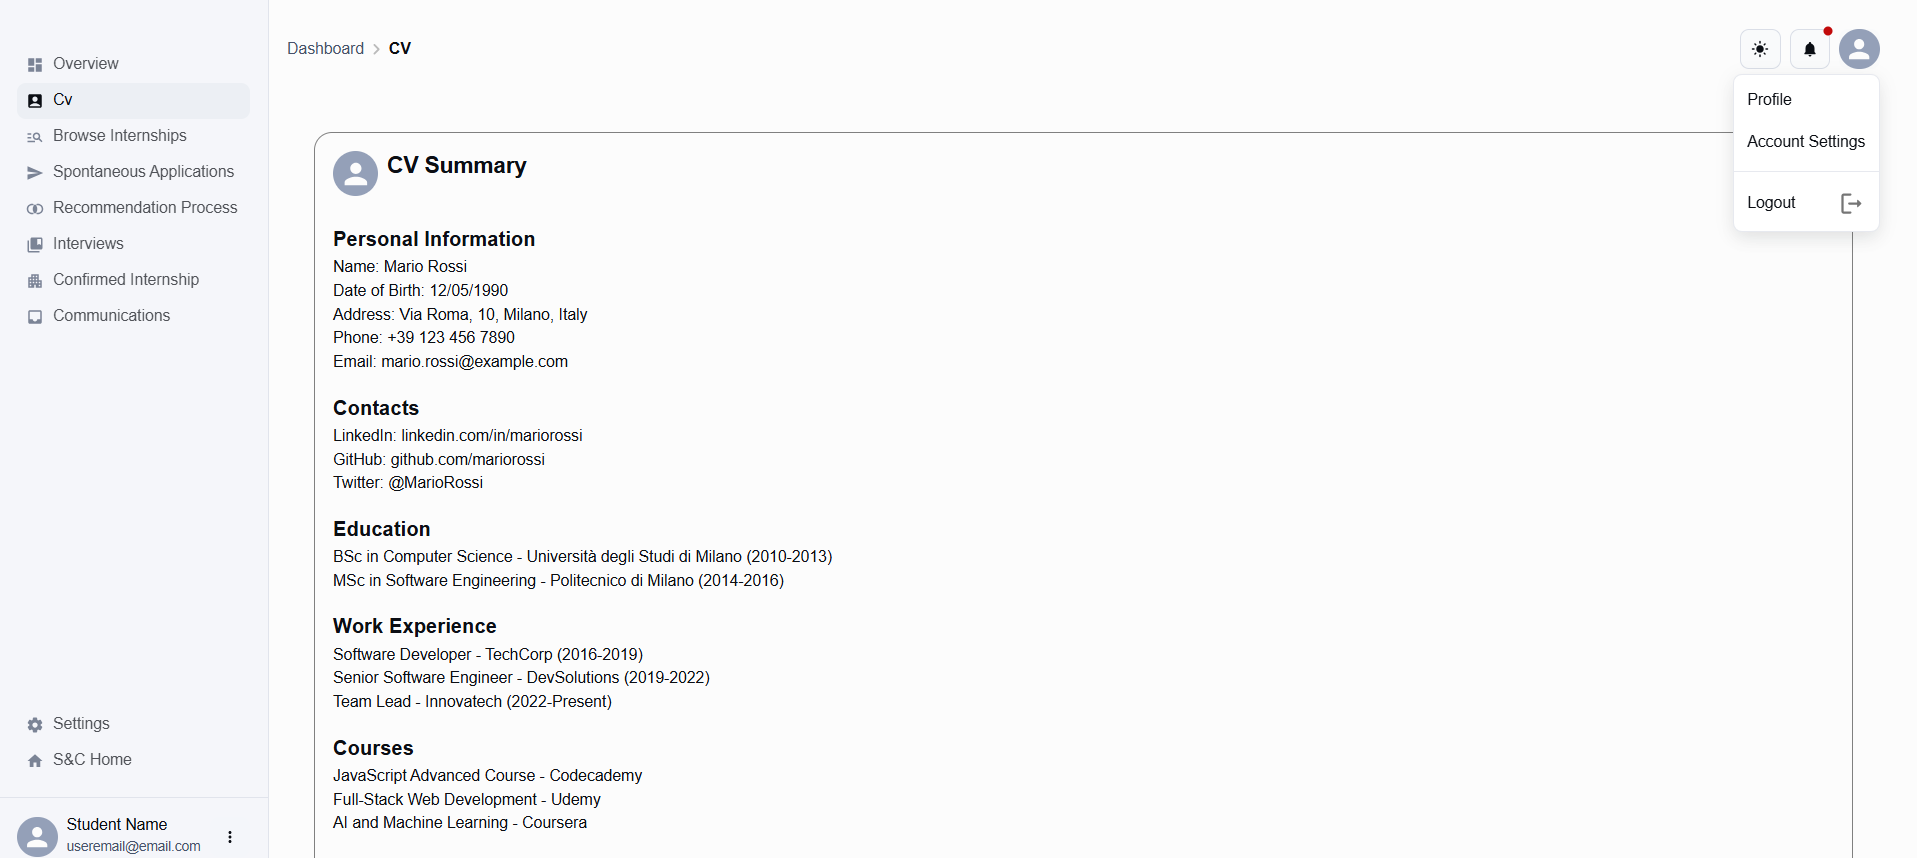
\includegraphics[width=\textwidth]{Latex/Images/New Ui/Student-Dashboard.png}
    \caption{UI Students Dashboard Page}
    \label{fig:studentDashboard}
\end{figure}
\begin{figure}[H]
    \centering
    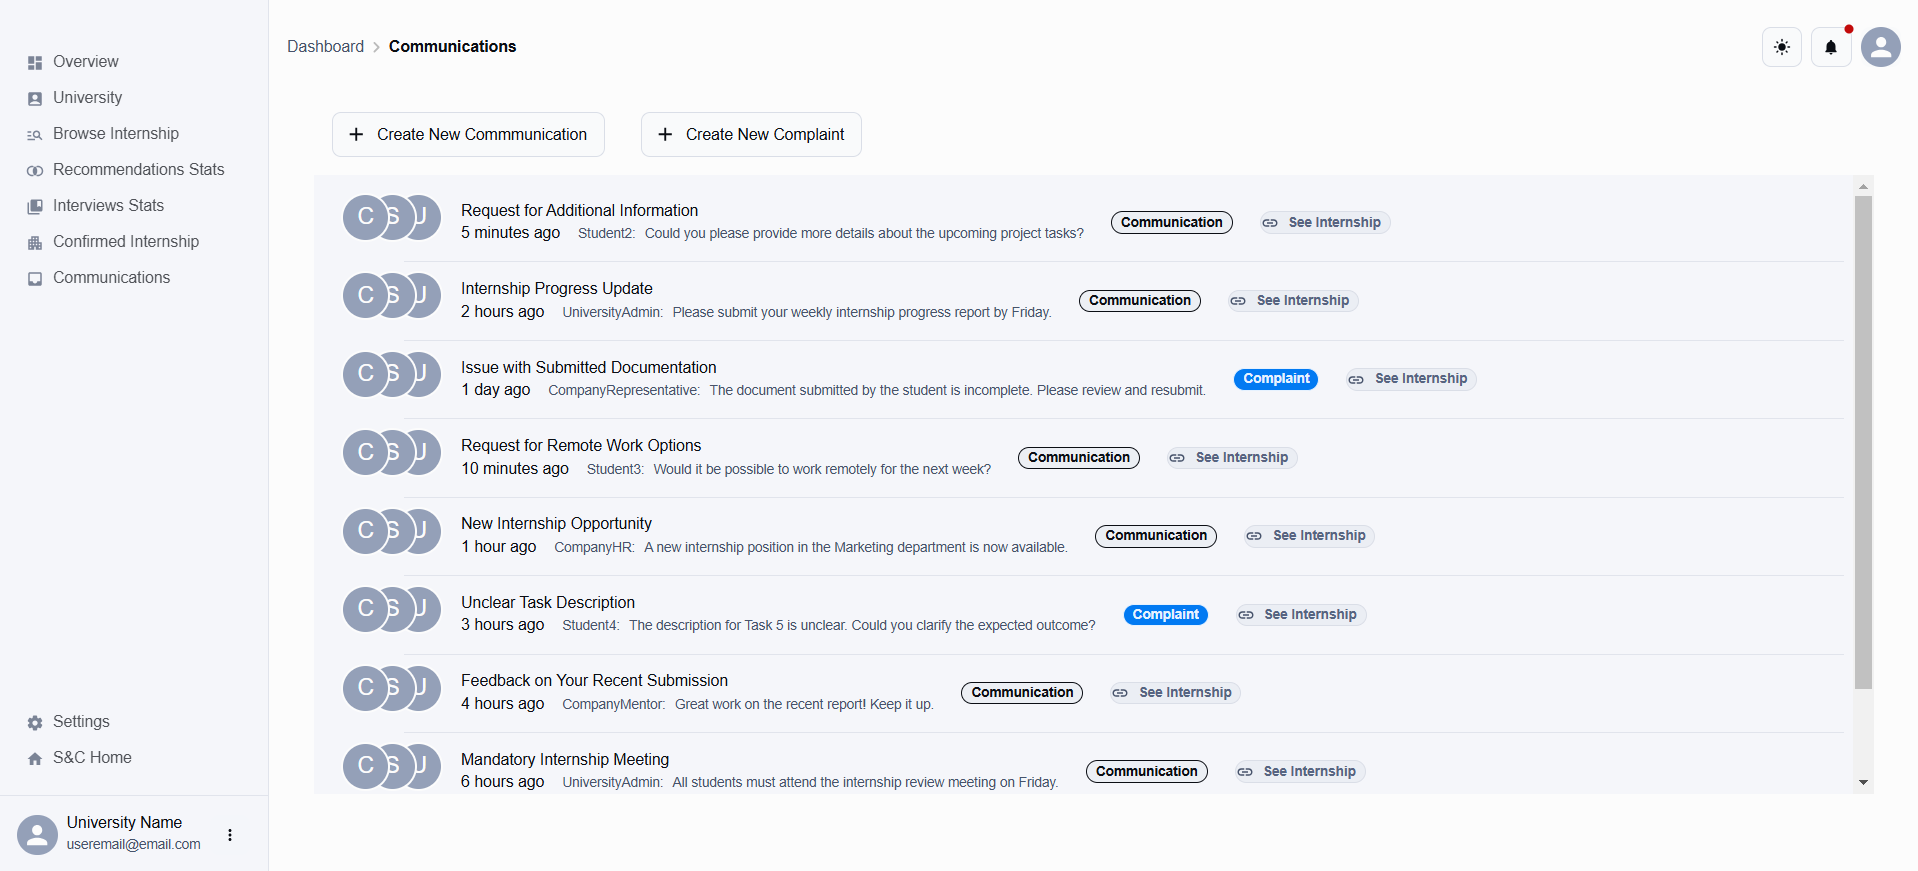
\includegraphics[width=\textwidth]{Latex/Images/New Ui/Uni-Dashboard.png}
    \caption{UI University Dashboard Page}
    \label{fig:universityDashboard}
\end{figure}